\chapter{Extreme-mass-ratio burst waveforms}\label{ch:waveforms}

\section{Massive black holes and extreme-mass-ratio events}

An exciting means of inferring information about MBHs is through GWs emitted when COs, such as stellar-mass BHs, NSs, WDs or low mass main sequence (MS) stars, pass close by \citep{Sathyaprakash2009}. A space-borne detector, such as LISA, is designed to be able to detect GWs in the frequency range of interest for these encounters \citep{Danzmann2003, Jennrich2011, Amaro-Seoane2012a}. The identification of waves requires a set of accurate waveform templates covering parameter space. Much work has already been done on the waveforms generated when companion objects inspiral towards an MBH \citep{Glampedakis2005, Barack2009}; as they orbit, the GWs carry away energy and angular momentum, causing the orbit to shrink until eventually the object plunges into the MBH. These systems are typically formed following two-body encounters so that the initial orbits are highly eccentric; a burst of radiation is emitted during each periapse passage. These are extreme mass-ratio bursts (EMRBs; \citealt{Rubbo2006}). Assuming that the companion is not scattered from its orbit, and does not plunge straight into the MBH, its orbit evolves, becoming more circular, and it shall begin to continuously emit significant gravitational radiation in the frequency range of a LISA-like space-borne detector. The resulting signals are extreme mass-ratio inspirals (EMRIs; \citealt{Amaro-Seoane2007}).

Studies of these systems have usually focused upon the phase when the orbit is close to plunge and completes a large number of cycles in the detector's frequency band, allowing a high signal-to-noise ratio (SNR) to be accumulated. Here, we investigate high eccentricity orbits. EMRBs are much shorter in duration than EMRIs; this means they do not accumulate as high SNRs, or produce as detailed maps of the spacetime. They are therefore less valued prizes. However, they may still be an interesting signal. As an object inspirals it emits many bursts before eventually settling into a low eccentricity EMRI. Some objects shall be scattered by two-body encounters and never reach the EMRI phase \citep{Alexander2003}. Thus, there are many potential EMRBs per EMRI, although this does not necessarily translate to there being more detectable EMRBs than EMRIs. The event rate for the detection of such EMRBs with LISA has been estimated to be as high as $15\units{yr^{-1}}$ \citep{Rubbo2006}, although this has been subsequently revised downwards to the order of $1\units{yr^{-1}}$ \citep{Hopman2007}. The event rate is dominated by bursts from the Galactic Centre (GC). Even if only a single burst is detected during a mission, this is still an exciting possibility since the information carried by the GW should give an unparalleled probe of the structure of spacetime of the GC.

To model bursts we make the simplifying assumption that all these orbits are marginally bound, or parabolic, since highly eccentric orbits appear almost indistinguishable from an appropriate parabolic orbit. Here ``parabolic'' and ``eccentricity'' refer to the energy of the geodesic and not to the geometric shape of the orbit.\footnote{Marginally bound Keplerian orbits (in flat spacetime) are parabolic in both senses.} Following such a trajectory an object may make just one pass of the MBH or, if the periapsis distance is small enough, it may complete a number of rotations. Such an orbit is referred to as zoom--whirl \citep{Glampedakis2002a}.

We begin our investigation of the properties of EMRBs as a means of studying MBHs by constructing approximate waveforms. To do so we integrate the geodesic equations for a parabolic orbit in Kerr spacetime (\secref{Geodesic}); we assume that the orbiting body is a test particle, such that it does not influence the underlying spacetime, and that the orbital parameters evolve negligibly during the orbit such that they may be held constant.\footnote{In \apref{evolve} it is shown that orbital evolution is typically negligible for EMR systems.} We use this trajectory to construct an approximate numerical kludge (NK) waveform \citep{Babak2007} as explained in \secref{Kludge}. In \secref{Signal} we establish what the LISA detectors would measure and how the signal would be analysed. Since there does not exist a definite mission design, we use the classic LISA design for the majority of this work. It is hoped that any future missions shall have comparable sensitivity, and studies using the LISA design are sensible benchmarks for comparison. In a few places we look at the detectability of bursts using eLISA, since this the currently most likely design for the first space-based detector. We confirm the accuracy of the kludge waveforms in \secref{Energy} by comparing the energy flux to fluxes calculated using other approaches. The typical error introduced by the NK approximation may be a few percent, but this worsens as the periapsis approaches the last non-plunging orbit.

Having established the accuracy of our NK waveforms, we study what information can be extracted from them. Exactly what can be inferred depends upon the orbit. We begin in \chapref{param} by looking at EMRBs from the GC as the Galaxy's MBH is the most promising to study. Finding promising results, we extend our study to extragalactic sources in \chapref{extragal}. We complete our analysis of EMRBs in \chapref{events}, where we build a simple model for burst event rates and use this to estimate what we could expect to learn from them.

\section{Parabolic orbits in Kerr spacetime}\label{sec:Geodesic}

\subsection{The metric and geodesic equations}

Astrophysical BHs are described by the Kerr metric \citep{Kerr1963}. In standard Boyer--Lindquist coordinates the line element is (\citealt{Boyer1967}; \citealt[section 13.7]{Hobson2006})
\begin{equation}
\dd s^2 = \dfrac{\varrho^2 \Delta}{\Sigma^2}c^2\dd t^2 - \dfrac{\Sigma \sin^2 \theta}{\varrho^2}\left(\dd \phi - \omega \dd t\right)^2 - \dfrac{\varrho^2}{\Delta}\dd r^2 - \varrho^2\dd \theta^2,
\end{equation}
where we have introduced functions
\begin{subequations}
\begin{align}
\varrho^2 = {} & r^2 + a^2\cos^2\theta,\\
\Delta = {} & r^2 - \dfrac{2GM_\bullet r}{c^2} + a^2,\\
\Sigma = {} & \left(r^2 +a^2\right)^2 - a^2\Delta\sin^2\theta,\\
\omega = {} & \dfrac{2GM_\bullet ar}{c\Sigma}.
\end{align}
\end{subequations}
For the remainder of this section we use natural units with $G = c = 1$.

Geodesics are parameterized by three conserved quantities (aside from the particle's mass $\mu$): energy (per unit mass) $E$, specific angular momentum about the symmetry axis (the $z$-axis) $L_z$, and Carter constant $Q$ (\citealt{Carter1968}; \citealt[section 62]{Chandrasekhar1992}). The geodesic equations are
\begin{subequations}
\begin{align}
\varrho^2 \diff{t}{\tau} = {} & a\left(L_z - aE\sin^2 \theta\right) + \dfrac{r^2 + a^2}{\Delta}\mathcal{T},\\
\varrho^2 \diff{r}{\tau} = {} & \pm \sqrt{V_r},\\
\varrho^2 \diff{\theta}{\tau} = {} & \pm \sqrt{V_\theta},\\
\varrho^2 \diff{\phi}{\tau} = {} & \dfrac{L_z}{\sin^2 \theta} - aE + \dfrac{a}{\Delta}\mathcal{T},
\end{align}
\end{subequations}
where we have introduced potentials
\begin{subequations}
\begin{align}
\mathcal{T} = {} & E\left(r^2 +a^2\right) - aL_z,\\
V_r = {} & \mathcal{T}^2 - \Delta\left[r^2 + \left(L_z - aE\right)^2 + Q\right],\\
V_\theta = {} & Q - \cos^2 \theta\left[a^2\left(1 - E^2\right) + \dfrac{L_z^2}{\sin^2\theta}\right],
\end{align}
\end{subequations}
and $\tau$ is proper time. The signs of the $r$ and $\theta$ equations can be chosen independently.

For a parabolic orbit $E = 1$; the particle is at rest at infinity. This simplifies the geodesic equations. It also allows us to give a simple interpretation for the Carter constant: this is defined as
\begin{equation}
Q = L_\theta^2 + \cos^2\theta\left[a^2\left(1 - E^2\right) + \dfrac{L_z^2}{\sin^2\theta}\right],
\end{equation}
where $L_\theta$ is the (non-conserved) specific angular momentum in the $\theta$-direction ($V_\theta = L_\theta^2$). For $E = 1$ we have
\begin{equation}
Q = L_\theta^2 + \cot^2\theta\, L_z^2 = L_\infty^2 - L_z^2;
\end{equation}
here $L_\infty$ is the total specific angular momentum at infinity, where the metric is asymptotically flat \citep{DeFelice1980}.\footnote{\citet{Rosquist2009} discuss the interpretation of $Q$ in the limit $G \rightarrow 0$, corresponding to a flat spacetime.} This is as in Schwarzschild spacetime.

\subsection{Integration variables and turning points}

In integrating the geodesic equations, difficulties can arise because of the presence of turning points, when the sign of the $r$ or $\theta$ geodesic equation changes. The radial turning points are at the periapsis $r\sub{p}$ and at infinity. We locate the periapsis by finding the roots of
\begin{align}
V_r = {} & 2M_\bullet r^3 - \left(L_z^2+Q\right)r^2 + 2M_\bullet\left[\left(L_z - a\right)^2 + Q\right]r - a^2 Q = {} 0.
\end{align}
This has three roots, which we shall denote $\{r_1, r_2, r\sub{p}\}$; the periapsis $r\sub{p}$ is the largest real root.\footnote{The apoapsis is not a (fourth) root to this equation as we have removed it by taking $E = 1$ before solving. This turning point can be found by setting the unconstrained expression for $V_r$ equal to zero, and then solving for $E(r)$; taking the limit $r \rightarrow \infty$ gives $E \rightarrow 1$ \citep{Wilkins1972}.}

We avoid the difficulties associated with the turning point by introducing angular variables that always increase with proper time \citep{Drasco2004}: inspired by Keplerian orbits, we parameterize our trajectory by
\begin{equation}
r = \dfrac{p}{1+e\cos\psi},
\end{equation}
where $e = 1$ is the eccentricity $p = 2r\sub{p}$ is the semilatus rectum and $\psi$ is the relativistic anomaly \citep{Darwin1961}. As $\psi$ covers its range from $-\pi$ to $\pi$, $r$ traces out a complete orbit. The geodesic equation for $\psi$ is
\begin{align}
\varrho^2 \diff{\psi}{\tau} = {} & \left\{M_\bullet\left[2r\sub{p} - \left(r_1 + r_2\right)\left(1 + \cos\psi\right) \vphantom{\dfrac{r_1 r_2}{2r\sub{p}}} +  \dfrac{r_1 r_2}{2r\sub{p}}\left(1 + \cos\psi\right)^2\right]\right\}^{1/2}.
\end{align}
Parameterizing an orbit by its periapsis and eccentricity has the additional benefit of allowing easier comparison with its flat-space equivalent \citep{Gair2005}.

The $\theta$ motion is usually bounded, with $\theta_- \leq \theta \leq \pi - \theta_-$; in the event that $L_z = 0$ the particle follows a polar orbit and $\theta$ covers its full range \citep{Wilkins1972}. The turning points are given by
\begin{equation}
V_\theta = Q - \cot^2\theta\, L_z^2 = 0.
\end{equation}
Changing variable to $\xi = \cos^2\theta$, we have a maximum value $\xi_- = \cos^2\theta_-$ given by
\begin{equation}
\xi_- = \dfrac{Q}{Q+L_z^2} = \dfrac{Q}{L_\infty^2}.
\label{eq:theta_0}
\end{equation}
See \figref{L_triangle} for a geometrical visualization.
\begin{figure}
\centering
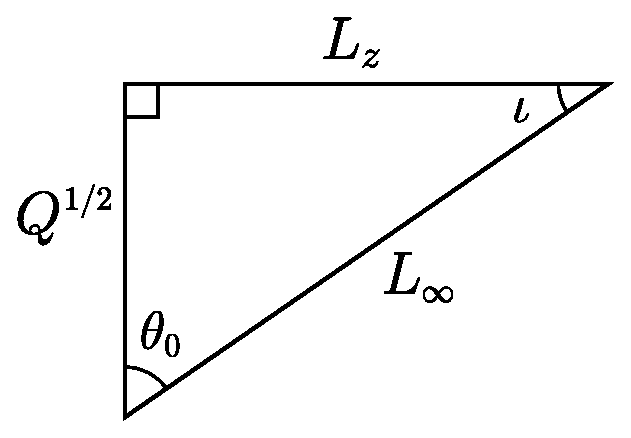
\includegraphics[width=0.25\textwidth]{./images/Triangle}
    \caption{The angular momenta $L_\infty$, $L_z$ and $\sqrt{Q}$ define a right-angled triangle. The acute angles are $\theta_-$, the extremal value of the polar angle, and $\iota$, the orbital inclination \citep{Ryan1996,Glampedakis2002}.}
    \label{fig:L_triangle}
\end{figure}
Introducing a second angular variable \citep{Hughes2000,Drasco2004}
\begin{equation}
\xi = \xi_-\cos^2\chi.
\end{equation}
Over one $2\pi$ period of $\chi$, $\theta$ oscillates from its minimum value to its maximum and back. The geodesic equation for $\chi$ is
\begin{equation}
\varrho^2\diff{\chi}{\tau} = \sqrt{Q + L_z^2}.
\end{equation}

\section{Waveform construction}\label{sec:Kludge}

We can now calculate the geodesic trajectory. The orbiting body is assumed to follow this track exactly; we ignore evolution due to the radiation of energy and angular momentum, which should be negligible for EMRBs as calculated in \apref{evolve}. From this trajectory we calculate the waveform using a semirelativistic approximation \citep{Ruffini1981}: we assume the particle moves along the Kerr geodesic, but radiates as if it were in flat spacetime. This quick-and-dirty technique is known as a numerical kludge (NK), and has been shown to approximate well results computed by more accurate methods \citep{Babak2007}. It is often compared to a bead travelling along a wire. The shape of the wire is set by the Kerr geodesic, but the bead moves along in flat space.

\subsection{The kludge approximation}

Numerical kludge approximations aim to encapsulate the main characteristics of a waveform by using the exact particle trajectory (ignoring inaccuracies from radiative effects and from the particle's self-force), whilst saving on computational time by using approximate waveform generation techniques.

We build an equivalent flat-space trajectory by identifying the Boyer--Lindquist coordinates with a set of flat-space coordinates. We consider two choices:
\begin{enumerate}
\item Identify the Boyer--Lindquist coordinates with flat-space spherical polars $\{r\sub{BL},$ $\theta\sub{BL},$ $\phi\sub{BL}\} \rightarrow \{r\sub{sph}, \theta\sub{sph}, \phi\sub{sph}\}$, then define flat-space Cartesian coordinates \citep{Gair2005, Babak2007}
\begin{equation}
\boldsymbol{x} = \begin{pmatrix}
r\sub{sph} \sin\theta\sub{sph}\cos\phi\sub{sph} \\
r\sub{sph} \sin\theta\sub{sph}\sin\phi\sub{sph} \\
r\sub{sph} \cos\theta\sub{sph}
\end{pmatrix}.
\end{equation}
\item Identify the Boyer--Lindquist coordinates with flat-space oblate-spheroidal coordinates \linebreak $\{r\sub{BL}, \theta\sub{BL}, \phi\sub{BL}\} \rightarrow \{r\sub{ob}, \theta\sub{ob}, \phi\sub{ob}\}$ so that the flat-space Cartesian coordinates are
\begin{equation}
\boldsymbol{x} = \begin{pmatrix}
\sqrt{{r\sub{ob}}^2 + a^2} \sin\theta\sub{ob}\cos\phi\sub{ob} \\
\sqrt{{r\sub{ob}}^2 + a^2} \sin\theta\sub{ob}\sin\phi\sub{ob} \\
r\sub{ob} \cos\theta\sub{ob}
\end{pmatrix}.
\end{equation}
These are appealing because in the limit that $G \rightarrow 0$, where the gravitating mass goes to zero, the Kerr metric in Boyer--Lindquist coordinates reduces to the Minkowski metric in oblate-spheroidal coordinates.
\end{enumerate}
The two coincide for $a \rightarrow 0$ or $r \rightarrow \infty$.

There is no well motivated argument that either coordinate system must yield an accurate GW; their use is justified {\it post facto} by comparison with results obtained from more accurate, and computationally intensive, methods \citep{Gair2005, Babak2007}. The ambiguity in assigning flat-space coordinates reflects the inconsistency of the semirelativistic approximation: the geodesic trajectory was calculated for the Kerr geometry; by moving to flat spacetime we lose the reason for its existence. This should not be regarded as a major problem; it is an artifact of the basic assumption that the shape of the trajectory is important for determining the character of the radiation, but the curvature of the spacetime in the vicinity of the source is not. By binding the particle to the exact geodesic, we ensure that the waveform has spectral components at the correct frequencies, but by assuming flat spacetime for generation of GWs they shall not have the correct amplitudes.

\subsection{The quadrupole--octupole formula}

Now we have a flat-space particle trajectory $x\sub{P}^\mu(\tau)$, we may apply a flat-space wave generation formula. We use the quadrupole--octupole formula to calculate the gravitational strain \citep{Bekenstein1973, Press1977, Yunes2008}
\begin{equation}
h^{jk}(t, \boldsymbol{x}) = -\dfrac{2G}{c^6r}\left(\ddot{I}^{jk} - 2n_i\ddot{S}^{ijk} + n_i\dddot{M}^{ijk}\right)_{t'\, =\, t - r/c},
\label{eq:octupole}
\end{equation}
where an over-dot represents differentiation with respect to time $t$, $t'$ is the retarded time, $r = \left|\boldsymbol{x} - \boldsymbol{x}\sub{P}\right|$ is the radial distance, $\boldsymbol{n}$ is the radial unit vector, and the mass quadrupole ${I}^{jk}$, current quadrupole ${S}^{ijk}$ and mass octupole ${M}^{ijk}$ are defined by
\begin{subequations}
\begin{align}
{I}^{jk}\left(t'\right) = {} & \intd{}{}{{x'}^j{x'}^kT^{00}\left(t', \boldsymbol{x'}\right) }{^3x'};\\
{S}^{ijk}\left(t'\right) = {} & \intd{}{}{{x'}^j{x'}^kT^{0i}\left(t', \boldsymbol{x'}\right)}{^3x'};\\
{M}^{ijk}\left(t'\right)  = {} & \recip{c}\intd{}{}{{x'}^i{x'}^j{x'}^kT^{00}\left(t', \boldsymbol{x'}\right)}{^3x'},
\end{align}
\end{subequations}
for energy-momentum tensor $T^{\mu\nu}$. This is correct for a slowly moving source. It is the familiar quadrupole formula \linebreak[0] (\citealt[section 36.10]{Misner1973}; \citealt[section 17.9]{Hobson2006}), derived from linearized theory, plus the next order terms. For a point mass, $T^{\mu\nu}$ contains a $\delta$-function which allows easy evaluation of the integrals.

Since we are only interested in GWs, we use the transverse-traceless (TT) gauge \citep[box 35.1]{Misner1973}.

\section{Signal detection and analysis}\label{sec:Signal}

\subsection{The LISA detector}\label{sec:Detector}

The classic LISA design is a three arm, space-borne laser interferometer \citep{Bender1998, Danzmann2003}. The arms form an equilateral triangle that rotates as the system's centre of mass follows a circular, heliocentric orbit, trailing $20^{\circ}$ behind the Earth. eLISA has a similar design, but  has only two arms, which are shorter in length, and trails $9^{\circ}$ behind the Earth \citep{Jennrich2011}.

To describe the detector configuration, and to transform from the MBH coordinate system to those of the detector, we use three coordinate systems: those of the BH at the GC $x_\bullet^i$; ecliptic coordinates centred at the solar system (SS) barycentre $x_\odot^i$, and coordinates that co-rotate with the detector $x\sub{d}^i$. The MBH's coordinate system and the SS coordinate system are depicted in \figref{BH_SS}.
\begin{figure}
\centering
 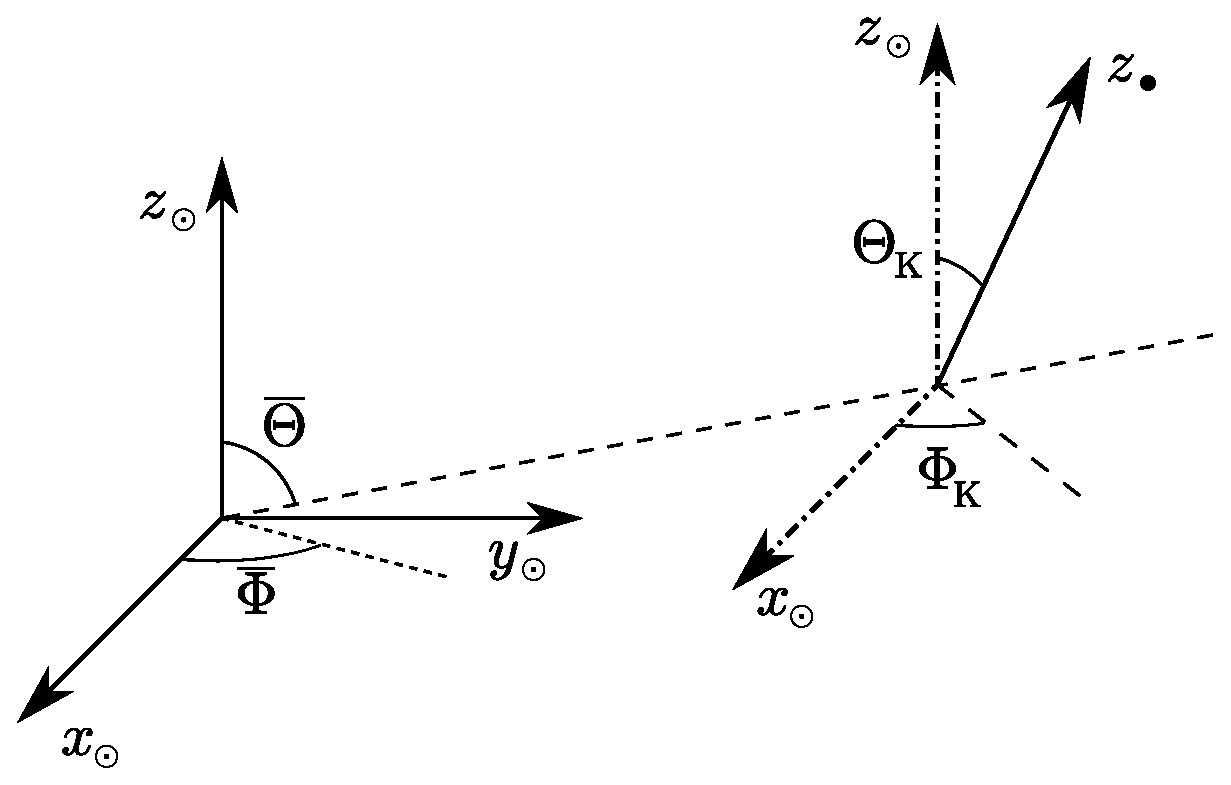
\includegraphics[width=0.42\textwidth]{./images/BH_SS_angles}
    \caption{The relationship between the MBH's coordinate system $x_\bullet^i$ and the SS coordinate system $x_\odot^i$. The MBH's spin axis is aligned with the $z_\bullet$-axis. The orientation of the MBH's $x$- and $y$-axes is arbitrary. We choose $x_\bullet$ to be orthogonal to the direction to the SS.}
   \label{fig:BH_SS}
\end{figure}
The mission geometry for LISA and eLISA is shown in \figref{SS_LISA}.
\begin{figure}
\centering
 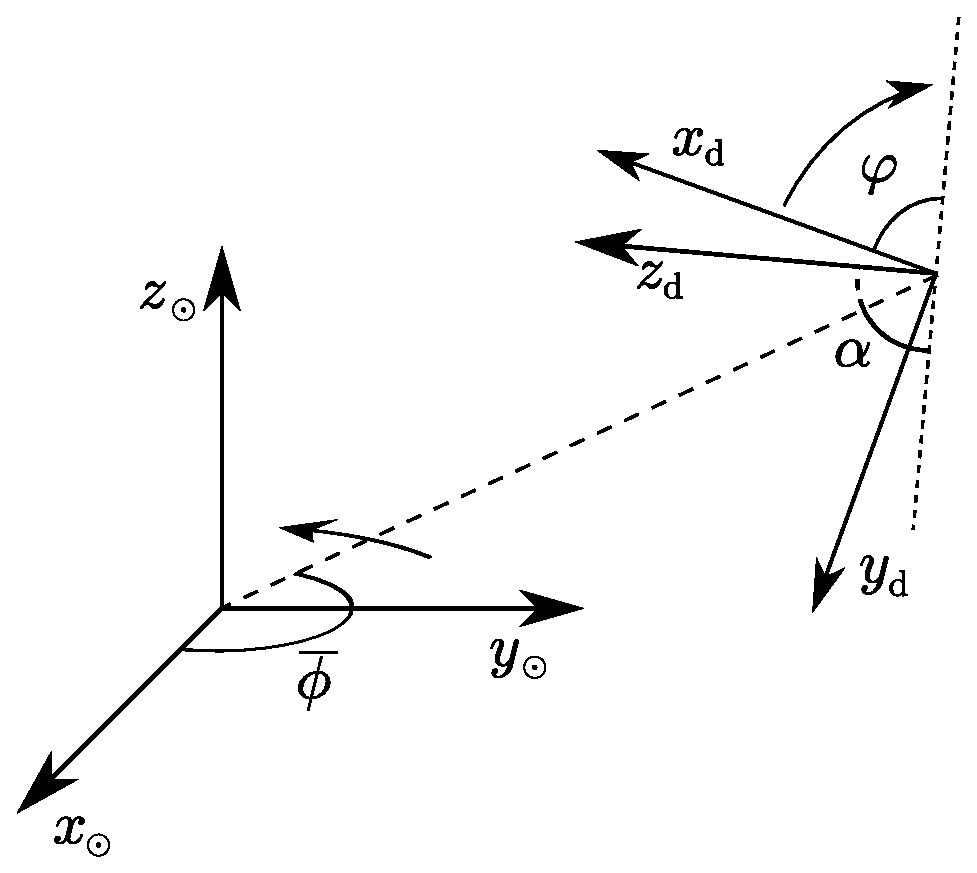
\includegraphics[width=0.32\textwidth]{./images/SS_LISA}
    \caption{The relationship between the detector coordinates $x\sub{d}^i$ and the ecliptic coordinates of the SS $x_\odot^i$ \citep{Bender1998, Jennrich2011}. The detector inclination is $\alpha = 60^{\circ}$.}
   \label{fig:SS_LISA}
\end{figure}
We define the detector coordinates such that the detector-arms lie in the $x\sub{d}$-$y\sub{d}$ plane as in \citet{Cutler1998}. We have computed the waveforms in the MBH's coordinates, but it is simplest to describe the measured signal using the detector's coordinates.

The strains measured in the three arms can be combined such that LISA behaves as a pair of $90^{\circ}$ interferometers at $45^{\circ}$ to each other, with signals scaled by ${\sqrt{3}}/{2}$ \citep{Cutler1998}. We denote the two detectors as I and II and use vector notation $\boldsymbol{h}(t) = \left(h\sub{I}(t), h\sub{II}(t)\right) = \left\{h_A(t)\right\}$ to represent signals from both detectors. As eLISA only has two arms it functions as a single detector, in this case $\left\{h_A(t)\right\} = h\sub{I}(t)$.

\subsection{Frequency domain formalism}

Having constructed the GW $\boldsymbol{h}(t)$ that shall be incident upon the detector, we may consider how to analyse the waveform and extract the information it contains. We briefly recap GW signal analysis, with application to LISA. A more complete discussion can be found in \citet{Finn1992} and \citet{Cutler1994}. Adaption for eLISA requires a substitution of the noise distribution, and the removal of the sum over data channels, since it would only have one.

The measured strain $\boldsymbol{s}(t)$ is the combination of the signal and the detector noise
\begin{equation}
\boldsymbol{s}(t) = \boldsymbol{h}(t) + \boldsymbol{n}(t);
\end{equation}
we assume the noise $n_A(t)$ is stationary and Gaussian, and that noise in the two detectors is uncorrelated, but shares the same characterisation \citep{Cutler1998}.

The properties of the noise allow us to define a natural inner product and associated distance on the space of signals \citep{Cutler1994}
\begin{equation}
\innerprod{\boldsymbol{g}}{\boldsymbol{k}} = 2\intd{0}{\infty}{\dfrac{\tilde{g}_A^\ast(f)\tilde{k}_A(f) + \tilde{g}_A(f)\tilde{k}_A^\ast(f)}{S_{n}(f)}}{f},
\label{eq:inner}
\end{equation}
introducing Fourier transforms
\begin{equation}
\tilde{g}(f) = \mathscr{F}\{g(t)\} = \intd{-\infty}{\infty}{g(t)\exp(2\pi i ft)}{t},
\end{equation}
and $S_{n}(f)$ is the noise spectral density. The inner product is derived in \apref{inner-prod}. The signal-to-noise ratio is approximately
\begin{equation}
\rho[\boldsymbol{h}] = \innerprod{\boldsymbol{h}}{\boldsymbol{h}}^{1/2}.
\label{eq:SNR}
\end{equation}
The probability of a particular realization of noise $\boldsymbol{n}(t) = \boldsymbol{n}_0(t)$ is
\begin{equation}
p(\boldsymbol{n}(t) = \boldsymbol{n}_0(t)) \propto \exp\left[-\recip{2}\innerprod{\boldsymbol{n}_0}{\boldsymbol{n}_0}\right].
\end{equation}
Thus, if the incident waveform is $\boldsymbol{h}(t)$, the probability of measuring signal $\boldsymbol{s}(t)$ is
\begin{equation}
p(\boldsymbol{s}(t)|\boldsymbol{h}(t)) \propto \exp\left[-\recip{2}\innerprod{\boldsymbol{s}-\boldsymbol{h}}{\boldsymbol{s}-\boldsymbol{h}}\right].
\label{eq:sig_prob}
\end{equation}

\subsection{The noise curve}\label{sec:Noise}

LISA's noise has two sources: instrumental noise and confusion noise, primarily from WD binaries. The latter may be divided into contributions from galactic and extragalactic binaries. In this work we use the noise model of \citet{Barack2004}. The shape of the noise curve can be seen in \figref{Noise}. The instrumental noise dominates at both high and low frequencies. The confusion noise is important at intermediate frequencies, and is responsible for the cusp around $10^{-3}\units{Hz}$. eLISA shares the same sources of noise, but is less affected by confusion \citep{Jennrich2011}. Its sensitivity regime is shifted to higher frequencies because of the shorter arm length.
\begin{figure}[!htp]
\centering
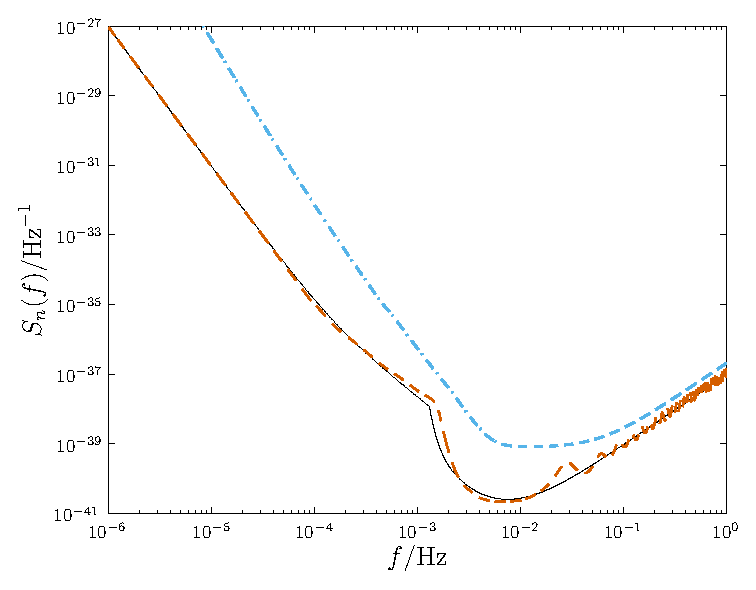
\includegraphics[width=0.6\textwidth]{./images/Fig_Noise}
\caption{The detector noise curves. The solid line indicates the analytic approximation of \citet{Barack2004} used in this work. For comparison, the dashed line is from the online LISA sensitivity curve generator (\url{http://www.srl.caltech.edu/~shane/sensitivity/}; \citealt*{Larson2000, Larson2002}). For bursts from the Galactic Centre we are most interested in the low-frequency region where the two curves are the same. The dot--dashed line shows the eLISA noise curve.}
\label{fig:Noise}
\end{figure}

\subsection{Window functions}

There is one remaining complication regarding signal analysis: as we are Fourier transforming a finite signal we encounter spectral leakage; a contribution from large amplitude spectral components leaks into surrounding components (sidelobes), obscuring and distorting the spectrum at these frequencies \citep{Harris1978}. This is an inherent problem with finite signals; it shall be as much of a problem when analysing signals from an actual mission as it is here. To mitigate, but unfortunately not eliminate, these effects, the time-domain signal can be multiplied by a window function. These are discussed in detail in \apref{window}. We adopt the Nuttall four-term window with continuous first derivative \citep{Nuttall1981} for our results. This should not affect the accuracy of our conclusions.

\section{Energy spectra}\label{sec:Energy}

To check the NK waveforms, we compare the energy spectra calculated from these with those obtained from the classic treatment of \citet{Peters1963} and \citet{Peters1964}. This calculates GW emission for Keplerian orbits in flat spacetime, assuming only quadrupole radiation. The spectrum produced should be similar to that obtained from the NK in weak fields, that is for large periapses; we do not expect an exact match because of the differing input physics and varying approximations.

In addition to using the energy spectrum, we also use the total energy flux. This contains less information than the spectrum; however, \citet{Martel2004} has calculated results for parabolic orbits in Schwarzschild spacetime using time-domain BH perturbation theory. These should be more accurate than results calculated using the Peters and Mathews formalism.

As we are considering Schwarzschild spacetime, the two NK coordinate choices coincide and there is no need to differentiate between them. In general, we do not intend to use the kludge waveforms to calculate an accurate energy flux: this would be inconsistent as we assume the orbits do not evolve with time. We only calculate the energy flux as a sanity check, to confirm that the kludge approximation is consistent with other approaches.

\subsection{Kludge spectrum}

A GW in the TT gauge has an effective energy-momentum tensor \citep[section 35.15]{Misner1973}
\begin{equation}
T_{\mu\nu} = \dfrac{c^4}{32\pi G}\left\langle\partial_\mu h_{ij} \partial_\nu h^{ij}\right\rangle,
\end{equation}
where $\langle\ldots\rangle$ indicates averaging over several wavelengths or periods. The energy flux through a sphere of radius $R$ is
\begin{equation}
\diff{E}{t} = \dfrac{c^3}{32\pi G} R^2 \int{\dd\Omega}\left\langle\diff{h_{ij}}{t}\diff{h^{ij}}{t}\right\rangle,
\end{equation}
with $\int{\dd\Omega}$ representing integration over all solid angles. From \eqnref{octupole} the waves have a $1/{r}$ dependence; if we define
\begin{equation}
h_{ij} = \dfrac{H_{ij}}{r},
\end{equation}
we see the flux is independent of $R$, as required for energy conservation, and
\begin{equation}
\diff{E}{t} = \dfrac{c^3}{32\pi G} \int{\dd\Omega}\left\langle\diff{H_{ij}}{t}\diff{H^{ij}}{t}\right\rangle.
\end{equation}
Integrating to find the total energy emitted
\begin{equation}
E = \dfrac{c^3}{32\pi G} \int{\dd\Omega}\int_{-\infty}^{\infty}{\dd t} \, \diff{H_{ij}}{t}\diff{H^{ij}}{t}.
\label{eq:integrate_E}
\end{equation}
Since we are considering all time, the localization of the energy is no longer of importance and it is unnecessary to average over several periods. Switching to Fourier representation $\widetilde{H}_{ij}(f) = \mathscr{F}\left\{H_{ij}(t)\right\}$,
\begin{equation}
E = \dfrac{\pi c^3}{4 G} \int{\dd\Omega}\int_{0}^{\infty}{\dd f} \, f^2 \widetilde{H}^{ij}(f)\widetilde{H}_{ij}^*(f),
\label{eq:total_E}
\end{equation}
using $\widetilde{H}_{ij}^*(f) = \widetilde{H}_{ij}(-f)$ as the signal is real. From this we identify the energy spectrum as
\begin{align}
\diff{E}{f} = \dfrac{\pi c^3}{4 G} \intd{}{}{}{\Omega} \, f^2 \widetilde{H}^{ij}(f)\widetilde{H}_{ij}^*(f).
\label{eq:NK_dEdf}
\end{align}

\subsection{Peters and Mathews spectrum}\label{sec:P-M}

For an orbit of eccentricity $e$ with periapse radius $r\sub{p}$, \citet{Peters1963} give the power radiated into the $n$-th harmonic of the orbital angular frequency as
\begin{equation}
P(n) = \dfrac{32}{5}\dfrac{G^4}{c^5}\dfrac{M_\bullet^2\mu^2(M_\bullet + \mu)(1-e)^5}{r\sub{p}^5}g(n,e),
\label{eq:PM_P}
\end{equation}
where the function $g(n,e)$ is defined in terms of Bessel functions of the first kind
\begin{align}
g(n,e) = {} & \dfrac{n^4}{32}\left\{\left[J_{n-2}(ne) - 2eJ_{n-1}(ne) + \dfrac{2}{n}J_n(ne) + 2eJ_{n+1}(ne) - J_{n+2}(ne)\right]^2 \right. \nonumber \\*
 & + \left. \left(1 - e^2\right)\left[J_{n-2}(ne) - 2J_n(ne) + J_{n+2}(ne)\right]^2 + \dfrac{4}{3n^2}\left[J_n(ne)\right]^2\right\}.
% Line breaks follow Peters and Mathews paper
\end{align}
The Keplerian orbital frequency is
\begin{equation}
\omega_1^2 = \dfrac{G(M_\bullet + \mu)(1 - e)^3}{r\sub{p}^3} = (1 - e)^3\omega\sub{c}^2,
\label{eq:Kepler_freq}
\end{equation}
where $\omega\sub{c}$ is defined as the angular frequency of a circular orbit of radius $r\sub{p}$. The energy radiated per orbit into the $n$-th harmonic, that is at frequency $\omega_n = n\omega_1$, is
\begin{equation}
E(n) = \dfrac{2\pi}{\omega_1}P(n);
\label{eq:E(n)}
\end{equation}
as $e \rightarrow 1$ for a parabolic orbit, $\omega_1 \rightarrow 0$ as the orbital period becomes infinite. The energy radiated per orbit is then the total energy radiated. The spacing of harmonics is $\Delta\omega = \omega_1$, giving energy spectrum
\begin{equation}
\left.\diff{E}{\omega}\right|_{\omega_n}\omega_1 = E(n).
\end{equation}
Changing to linear frequency $2\pi f = \omega$,
\begin{align}
\left.\diff{E}{f}\right|_{f_n}  = {} & \dfrac{128\pi^2}{5}\dfrac{G^3}{c^5}\dfrac{M_\bullet^2\mu^2}{r\sub{p}^2}(1-e)^2g(n,e) \\*
  = {} & \dfrac{4\pi^2}{5}\dfrac{G^3}{c^5}\dfrac{M_\bullet^2\mu^2}{r\sub{p}^2}\ell(n,e),
\label{eq:PM_spectrum}
\end{align}
where the function $\ell(n,e)$ is defined in the last line. For a parabolic orbit, we must take the limit of $\ell(n,e)$ as $e \rightarrow 1$.

We simplify $\ell(n,e)$ using the recurrence formulae \citep[section 2.12]{Watson1995}
\begin{align}
J_{\nu-1}(z) + J_{\nu+1}(z)  = {} & \dfrac{2\nu}{z}J_\nu(z)\\*
J_{\nu-1}(z) - J_{\nu+1}(z)  = {} & 2J'_\nu(z),\label{eq:J_derivative}
\end{align}
and eliminate $n$ using
\begin{equation}
n = \dfrac{\omega_n}{\omega_1} = (1-e)^{-3/2}\tilde{f},
\end{equation}
where $\tilde{f} = \omega_n/\omega\sub{c} = f_n/f\sub{c}$ is a dimensionless frequency. To find the limit we define two new functions \citep{Berry2010}
\begin{equation}
A(\tilde{f}) = \lim_{e\rightarrow 1}\left\{\dfrac{J_n(ne)}{(1-e)^{1/2}}\right\}; \quad B(\tilde{f}) = \lim_{e\rightarrow 1}\left\{\dfrac{J'_n(ne)}{1-e}\right\}.
\end{equation}
To give a well-defined energy spectrum, both of these must be finite.

The Bessel function has an integral representation
\begin{equation}
J_\nu(z) = \recip{\pi}\intd{0}{\pi}{\cos(\nu\vartheta - z\sin\vartheta)}{\vartheta};
\end{equation}
we want the limit of this for $\nu \rightarrow \infty$, $z \rightarrow \infty$, with $z \leq \nu$. Using the stationary phase approximation, the dominant contribution to the integral comes from the regime in which the argument of the cosine is approximately zero \citep[sections 8.2, 8.43]{Watson1995}:
\begin{align}
J_\nu(z)  \sim {} & \recip{\pi}\intd{0}{\pi}{\cos\left(\nu\vartheta - z\vartheta + \dfrac{z}{6}\vartheta^3\right)}{\vartheta}\\*
  \sim {} & \recip{\pi}\intd{0}{\infty}{\cos\left(\nu\vartheta - z\vartheta + \dfrac{z}{6}\vartheta^3\right)}{\vartheta};
\end{align}
this last expression is an Airy integral and has a standard form \citep[section 6.4]{Watson1995}
\begin{equation}
\intd{0}{\infty}{\cos(t^3 + xt)}{t} = \dfrac{\sqrt{x}}{3}K_{1/3}\left(\dfrac{2x^{3/2}}{3^{3/2}}\right),
\end{equation}
where $K_\nu(z)$ is a modified Bessel function of the second kind. Using this to evaluate the limit gives
\begin{equation}
J_\nu(z) \sim \recip{\pi}\sqrt{\dfrac{2(\nu - z)}{3z}}K_{1/3}\left(\dfrac{2^{3/2}}{3}\sqrt{\dfrac{(\nu -z)^3}{z}}\right).
\label{eq:J_nu}
\end{equation}
For our case,
\begin{equation}
J_n(ne) \sim \recip{\pi}\sqrt{\dfrac{2}{3}}(1-e)^{1/2}K_{1/3}\left(\dfrac{2^{3/2}\tilde{f}}{3}\right),
\end{equation}
and the first limiting function is well defined,
\begin{equation}
A(\tilde{f}) = \recip{\pi}\sqrt{\dfrac{2}{3}}K_{1/3}\left(\dfrac{2^{3/2}\tilde{f}}{3}\right).
\end{equation}

To find the derivative we combine equations \eqref{eq:J_derivative} and \eqref{eq:J_nu}, and expand to lowest order yielding
\begin{align}
J'_n(ne) \sim {} & -\dfrac{1}{2\pi}\sqrt{\dfrac{2}{3}}(1-e)\left[2^{3/2}K'_{1/3}\left(\dfrac{2^{3/2}\tilde{f}}{3}\right) + \recip{\tilde{f}}K_{1/3}\left(\dfrac{2^{3/2}\tilde{f}}{3}\right)\right].
\end{align}
We may re-express the derivative using the recurrence formula \citep[section 3.71]{Watson1995}
\begin{equation}
K_{\nu-1}(z) + K_{\nu+1}(z) = -2K'_\nu(z)
\end{equation}
to give
\begin{align}
J'_n(ne)  \sim {} & \dfrac{1-e}{\sqrt{3}\pi}\left[K_{-2/3}\left(\dfrac{2^{3/2}\tilde{f}}{3}\right) + K_{4/3}\left(\dfrac{2^{3/2}\tilde{f}}{3}\right) - \recip{\sqrt{2}\tilde{f}}K_{1/3}\left(\dfrac{2^{3/2}\tilde{f}}{3}\right)\right].
\end{align}
And so finally we obtain the well-defined
\begin{align}
B(\tilde{f})  = {} & \recip{\sqrt{3}\pi}\left[K_{-2/3}\left(\dfrac{2^{3/2}\tilde{f}}{3}\right) + K_{4/3}\left(\dfrac{2^{3/2}\tilde{f}}{3}\right) - \recip{\sqrt{2}\tilde{f}}K_{1/3}\left(\dfrac{2^{3/2}\tilde{f}}{3}\right)\right].
\end{align}

Having obtained expressions for $A(\tilde{f})$ and $B(\tilde{f})$ in terms of standard functions, we can calculate the energy spectrum for a parabolic orbit. From \eqnref{PM_spectrum}
\begin{equation}
\diff{E}{f} = \dfrac{4\pi^2}{5}\dfrac{G^3}{c^5}\dfrac{M_\bullet^2\mu^2}{r\sub{p}^2}\ell\left(\dfrac{f}{f\sub{c}}\right),
\label{eq:PM_dEdf}
\end{equation}
where we have used the limit
\begin{align}
\ell(\tilde{f})  = {} & \left[8\tilde{f}^2B(\tilde{f}) - 2\tilde{f}A(\tilde{f})\right]^2 + \left(128\tilde{f}^4 + \dfrac{4\tilde{f}^2}{3}\right)\left[A(\tilde{f})\right]^2.
\label{eq:ell}
\end{align}
This agrees with the $e = 1$ result of \citet{Turner1977}, which was computed by direct integration along unbound orbits. \Figref{ell} shows how $\ell(n,e)$ changes with eccentricity including our result for a parabolic encounter. Although more power is radiated into higher harmonics, the peak of the spectrum does not move much: it is always between $f = f\sub{c}$ and $f = 2 f\sub{c}$, with $f = 2 f\sub{c}$ for $e = 0$ and $f \simeq 1.637 f\sub{c}$ for $e = 1$.
\begin{figure}%[!htp]
\centering
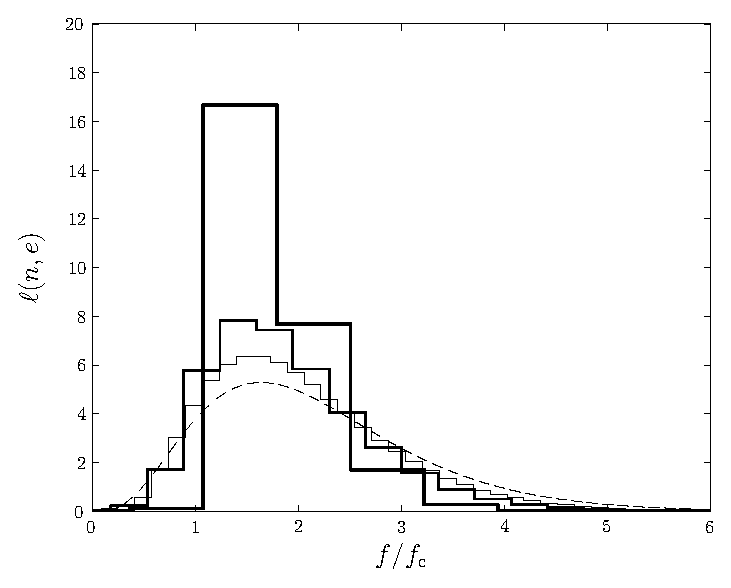
\includegraphics[width=0.6\textwidth]{./images/Fig_ell}
\caption{The relative energy (per orbit) spectrum $\ell(n,e)$ for $e = 0.2$ (heavy line), $e = 0.5$ (medium line), $e = 0.7$ (light line), and the limiting result for $e = 1$ (dashed line) versus frequency. Compare with figure 3 of \citet{Peters1963}.}
\label{fig:ell}
\end{figure}

\subsubsection{Total Energy}

To check the validity of this limit we can calculate the total energy radiated by integrating \eqnref{PM_dEdf} over all frequencies, or by summing the energy radiated into each harmonic. These must yield the same result. Summing:
\begin{equation}
E\sub{sum} = \dfrac{64\pi}{5}\dfrac{G^3}{c^5}\dfrac{M_\bullet^2\mu^2}{r\sub{p}^2}\omega\sub{c}(1-e)^{7/2}\sum_n g(n,e),
\end{equation}
where we have used equations \eqref{eq:PM_P}, \eqref{eq:Kepler_freq} and \eqref{eq:E(n)}. \citet{Peters1963} provide the result
\begin{equation}
\sum_n g(n,e) = \dfrac{1 + (73/24)e^2 + (37/96)e^4}{(1-e^2)^{7/2}}.
\end{equation}
Using this,
\begin{equation}
E\sub{sum} = \dfrac{64\pi}{5}\dfrac{G^3}{c^5}\dfrac{M_\bullet^2\mu^2}{r\sub{p}^2}\omega\sub{c}\dfrac{1 + (73/24)e^2 + (37/96)e^4}{(1+e)^{7/2}},
\end{equation}
which is perfectly well behaved as $e \rightarrow 1$,
\begin{equation}
E\sub{sum} = \dfrac{85\pi}{2^{5/2}3}\dfrac{G^3}{c^5}\dfrac{M_\bullet^2\mu^2}{r\sub{p}^2}\omega\sub{c}.
\label{eq:PM_total}
\end{equation}
Integrating the energy spectrum \eqnref{PM_dEdf} gives
\begin{equation}
E\sub{int} = \dfrac{2\pi}{5}\dfrac{G^3}{c^5}\dfrac{M_\bullet^2\mu^2}{r\sub{p}^2}\omega\sub{c}\intd{0}{\infty}{\ell(\tilde{f})}{\tilde{f}}.
\end{equation}
The integral can be evaluated numerically as
\begin{equation}
\intd{0}{\infty}{\ell(\tilde{f})}{\tilde{f}} = 12.5216858\ldots = \dfrac{425}{2^{7/2}3}.
\end{equation}
The two total energies are consistent, $E\sub{int} = E\sub{sum}$.

\subsection{Comparison}

Two energy spectra are plotted in \figref{Energy} for orbits with periapses of $r\sub{p} = 15.0 r\sub{g}$, $30.0 r\sub{g}$ and $60.0 r\sub{g}$.
\begin{figure}%[!htp]
  \centering
   \subfigure[$r\sub{p} = 15.0 r\sub{g}$, log-log plot.]{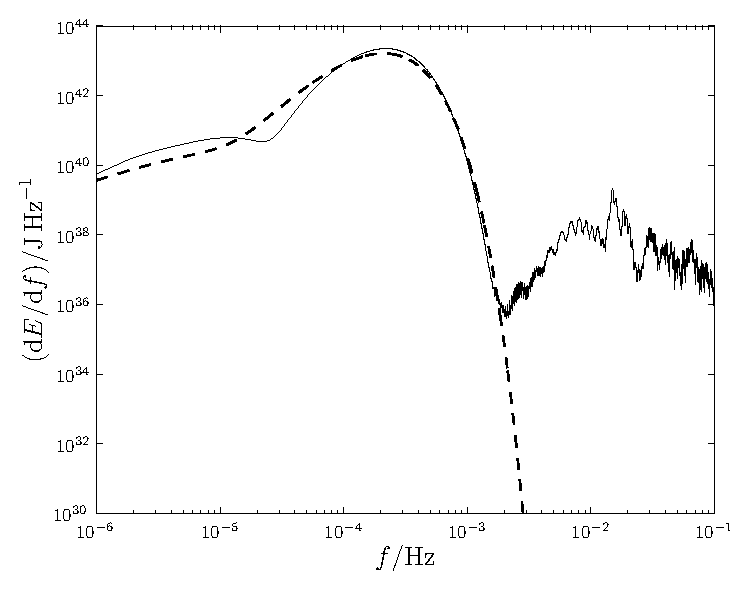
\includegraphics[width=0.48\textwidth]{./images/Fig_Loglog_E_15}} \quad
   \subfigure[$r\sub{p} = 15.0 r\sub{g}$, log-linear plot.]{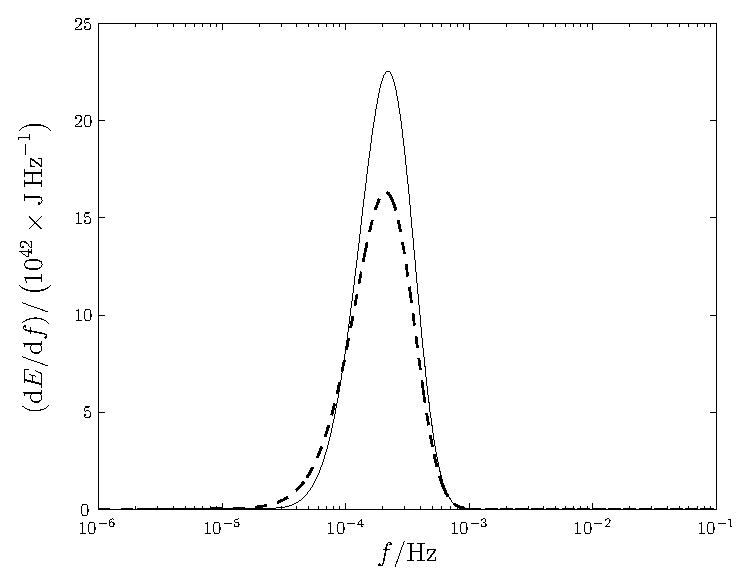
\includegraphics[width=0.48\textwidth]{./images/Fig_Loglin_E_15}} \\
   \subfigure[$r\sub{p} = 30.0 r\sub{g}$, log-log plot.]{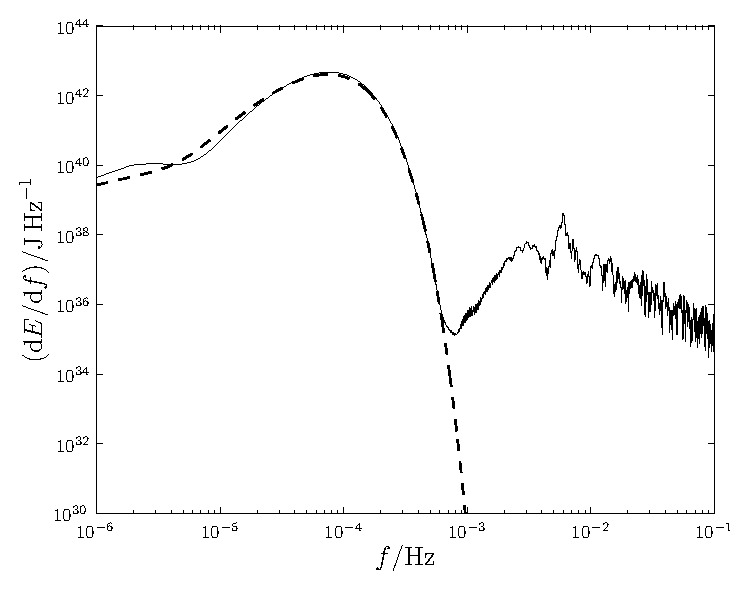
\includegraphics[width=0.48\textwidth]{./images/Fig_Loglog_E_30}} \quad
   \subfigure[$r\sub{p} = 30.0 r\sub{g}$, log-linear plot.]{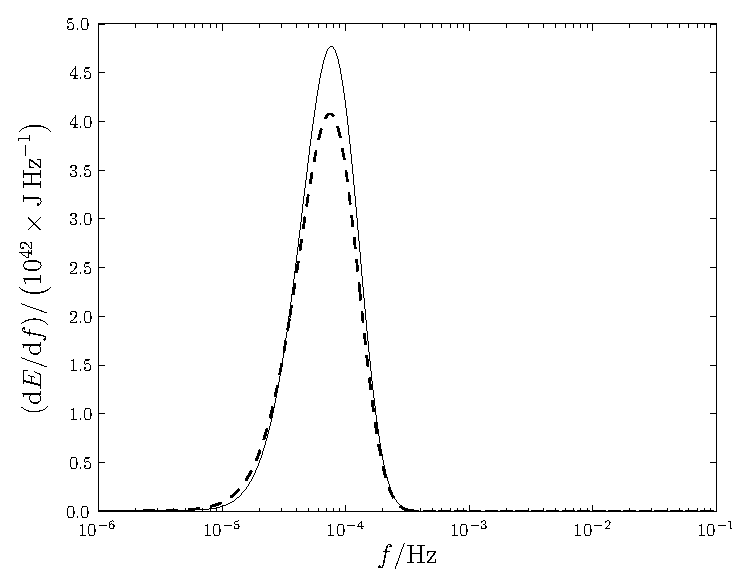
\includegraphics[width=0.48\textwidth]{./images/Fig_Loglin_E_30}} \\
   \subfigure[$r\sub{p} = 60.0 r\sub{g}$, log-log plot.]{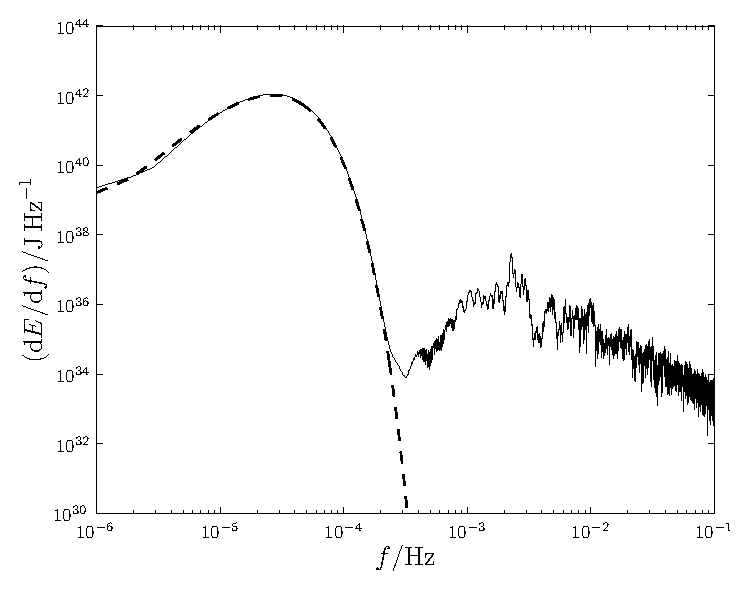
\includegraphics[width=0.48\textwidth]{./images/Fig_Loglog_E_60}} \quad
   \subfigure[$r\sub{p} = 60.0 r\sub{g}$, log-linear plot.]{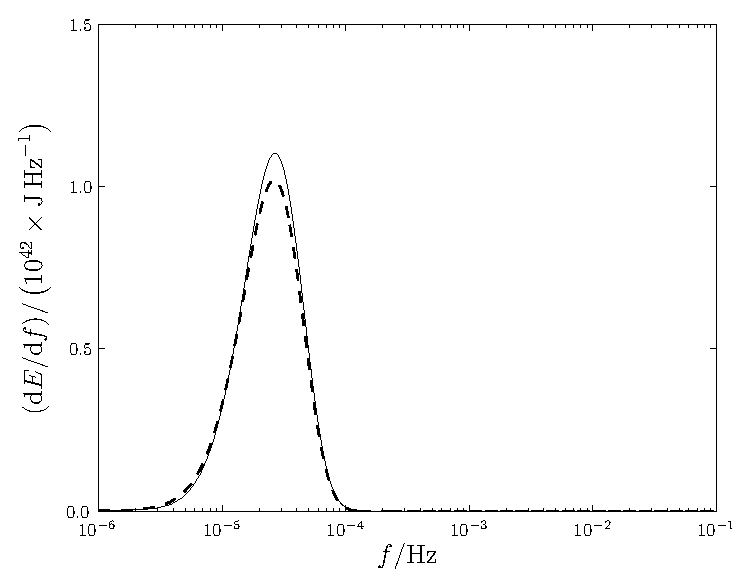
\includegraphics[width=0.48\textwidth]{./images/Fig_Loglin_E_60}}
    \caption{Energy spectra for a parabolic orbit of a $\mu = 10 M_\odot$ object about a Schwarzschild BH with $M_\bullet = 4.31 \times 10^6 M_\odot$. The spectra calculated from the NK waveform is shown by the solid line and the Peters and Mathews flux is indicated by the dashed line. The NK waveform includes octupole contributions. The high frequency tail is the result of spectral leakage.}
    \label{fig:Energy}
\end{figure}
The two spectra appear to be in good agreement, showing the same general shape in the weak-field limit. The NK spectrum is more tightly peaked, but is always within a factor of $2$ at the apex. The peak of the spectrum is shifted to a marginally higher frequency in the NK spectrum primarily because of the addition of the current quadrupole and mass octupole terms.

Comparing the total energy fluxes, ratios of the various energies are plotted in \figref{Energy_ratio}.
\begin{figure}%[!htp]
  \centering
   \subfigure[Versus periapsis]{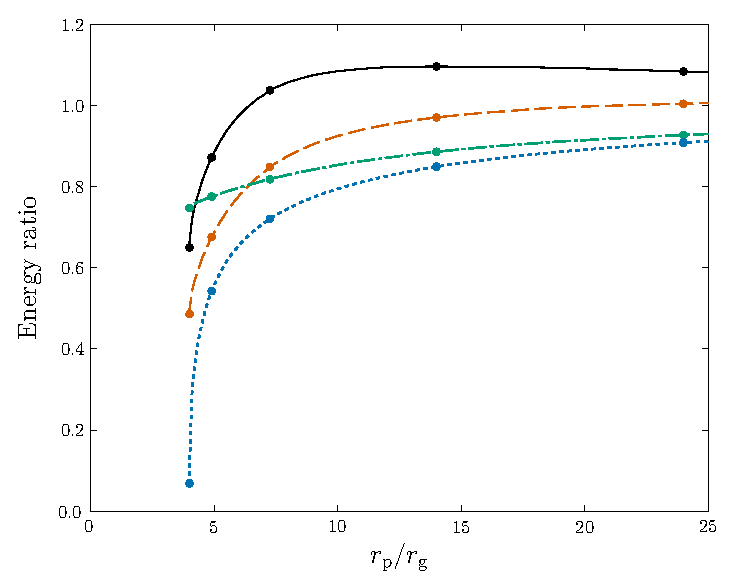
\includegraphics[width=0.475\textwidth]{./images/Fig_Energy_ratio_peri}} \quad
   \subfigure[Versus amount of rotation]{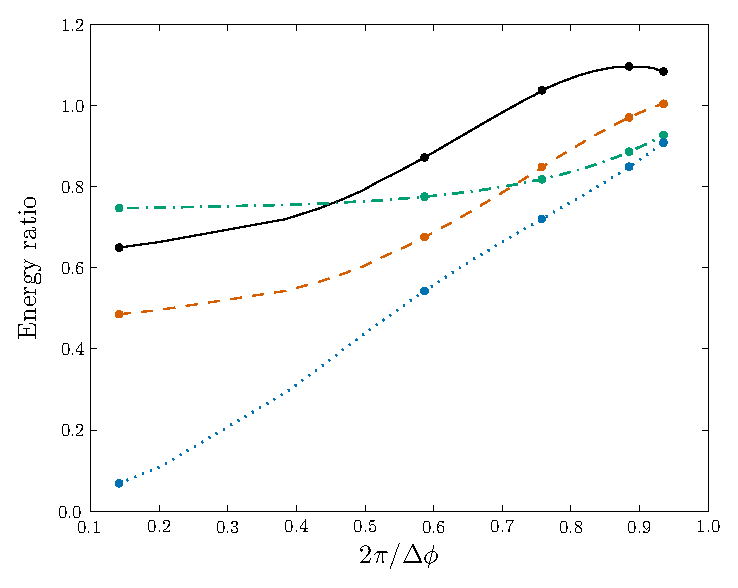
\includegraphics[width=0.475\textwidth]{./images/Fig_Energy_ratio_orbit}}
    \caption{Ratios of energies as a function of periapsis $r\sub{p}$ and $2\pi$ divided by the total angle of rotation in one orbit $\Delta\phi$ ($2\pi/\Delta\phi = 1$ for a Keplerian orbit). The solid line shows the ratio of the numerical kludge and Martel energies $E\sub{NK}/E\sub{M}$; the dashed line shows the ratio of the NK energy calculated using only the mass quadrupole term and the Martel energy $E\sub{NK(Q)}/E\sub{M}$; the dot--dashed line shows the ratio of the quadrupole and quadrupole--octupole NK energies $E\sub{NK(Q)}/E\sub{NK}$, and the dotted line shows the ratio of the Peters and Mathews and quadrupole NK energies $E\sub{PM}/E\sub{NK(Q)}$. The spots show the mapping between the two abscissa scales. Compare with figure 4 of \citet{Gair2005}.}
  \label{fig:Energy_ratio}
\end{figure}
We introduce an additional energy here, the quadrupole NK energy $E\sub{NK(Q)}$. This allows easier comparison with the Peters and Mathews energy which includes only quadrupole radiation. It can be calculated in three ways:
\begin{enumerate}
\item Inserting the waveform $\widetilde{h}(f)$ generated including only the mass quadrupole term in \eqnref{octupole} into \eqnref{total_E} and integrating. This is equivalent to the method used to calculate $E\sub{NK}$.
\item Numerically integrating the quadrupole GW luminosity (\citealt{Misner1973}, section 36.7; \citealt{Hobson2006}, section 18.7)
\begin{equation}
E = \dfrac{G}{5c^9}\intd{}{}{\dddot{\Ibar}_{ij}\dddot{\Ibar}^{ij}}{t},
\label{eq:E_quad}
\end{equation}
where $\Ibar_{ij} = I_{ij} - (1/3)I\delta_{ij}$ is the reduced mass quadrupole tensor. We can obtain this from \eqnref{integrate_E}, by integrating over all angles when the waveform only contains the mass quadrupole component. This has the advantage of avoiding the effects of spectral leakage or the influence of window functions.
\item Using the analytic expressions for the integral \eqnref{E_quad} from appendix A of \citet{Gair2005}. The expressions are included in \apref{energy}.
\end{enumerate}
All three agree to within computational error. No difference is visible on the scale plotted in \figref{Energy_ratio}. This demonstrates the validity of the code.

We have used the amount of rotation $\Delta\phi$ as a convenient measure for the abscissa. For an equatorial orbit in Kerr spacetime,
\begin{align}
\Delta\phi  = {} & 2\intd{r\sub{p}}{\infty}{\diff{\phi}{r}}{r} = \sqrt{\dfrac{2}{M_\bullet}}L_z\intd{r\sub{p}}{\infty}{\dfrac{r^2 - 2M_\bullet(1 - a/L_z)r}{(r^2 - 2M_\bullet r + a^2)w}}{r},
\end{align}
where
\begin{equation}
w^2 = r^3 - \dfrac{L_z^2}{2M_\bullet}r^2 + (L_z - a)^2r;
\end{equation}
$L_z$ is the specific angular momentum about the $z$-axis; $a$ is the spin parameter, and we have adopted units with $G = c = 1$. We shall find it useful to define
\begin{equation}
r_\pm = M_\bullet \pm \sqrt{M_\bullet^2 - a^2},
\end{equation}
and the two nonzero roots of the cubic $w^2$
\begin{equation}
r_{\mathrm{p},\,1} = \dfrac{L_z^2}{4M_\bullet} \pm \sqrt{\dfrac{L_z^4}{16M_\bullet^2} - (L_z -a)^2};
\end{equation}
the periapsis is the larger root $r\sub{p} > r_1$. This equation implicitly gives $L_z$ as a function of $r\sub{p}$. The integral may be rewritten as
\begin{equation}
\Delta\phi = \sqrt{\dfrac{2}{M}}L_z\intd{r\sub{p}}{\infty}{\recip{w}\left(1 + \dfrac{\alpha_+}{r-r_+} + \dfrac{\alpha_-}{r-r_-}\right)}{r},
\end{equation}
where
\begin{equation}
\alpha_\pm = \pm\dfrac{2Mar_\pm - a^2L_z}{2L_z\sqrt{M^2-a^2}}.
\end{equation}
This may be evaluated using elliptic integrals \citep[3.131.8, 3.137.8]{Gradshteyn2000}
\begin{equation}
\Delta\phi = 2 L_z \sqrt{\dfrac{2}{r\sub{p}M}}\left[\dfrac{\alpha_+}{r_+}\Pi\left(\dfrac{r_+}{r\sub{p}}\middle|\dfrac{r_1}{r\sub{p}}\right) + \dfrac{\alpha_-}{r_-}\Pi\left(\dfrac{r_-}{r\sub{p}}\middle|\dfrac{r_1}{r\sub{p}}\right)\right],
\end{equation}
where $\Pi(n|m) = \int_{0}^{\pi/2}{\dd\vartheta/(1-n\sin^2\vartheta)\sqrt{1-m\sin^2\vartheta}}$ is the complete elliptic integral of the third kind. In the limit of $a \rightarrow 0$ we recover the Schwarzschild result \citep{Cutler1994}
\begin{equation}
\Delta\phi =  2 L_z\sqrt{\dfrac{2}{r\sub{p}M}}K\left(\dfrac{r_1}{r\sub{p}}\right),
\end{equation}
where $K(m) = \int_{0}^{\pi/2}{\dd\vartheta/\sqrt{1-m\sin^2\vartheta}}$ is the complete elliptic integral of the first kind.

The ratios all tend towards one in the weak field, as required, but differences become more pronounced in the strong field. The NK energy is larger than the Peters and Mathews result $E\sub{PM}$. This behaviour has been seen before for high eccentricity orbits about a non-spinning BH \citep{Gair2005}. It may be explained by considering the total path length for the different orbits: the Peters and Mathews spectrum assumes a Keplerian orbit, the orbit in Kerr geometry rotates more than this. The greater path length leads to increased emission of GWs and a larger energy flux. Our bead must travel further along its wire. A good proxy for the path length is the angle of rotation $\Delta\phi$; this is $2\pi$ for a Keplerian orbit, in Kerr the angle should be $2\pi$ in the limit of an infinite periapsis, whereas for a periapsis small enough that the orbit shows zoom--whirl behaviour, the total angle may be many times $2\pi$. There is a reasonable correlation between the amount of rotation $2\pi/\Delta\phi$ and the ratio of energies.

Error in the NK energy compared with the time-domain BH perturbation theory results of Martel comes from two sources: the neglecting of higher order multipole contributions and the ignoring of background curvature. The contribution of the former can be estimated by looking at the difference in the NK energy by including the current quadrupole and mass octupole terms. From \figref{Energy_ratio} we see that these terms give a negligible contribution in the weak field, but the difference is $\sim20\%$ in the strong field. This explains why the Martel energy $E\sub{M}$ is greater in the strong field, as it includes contributions from all multipoles. Neglecting the background curvature increases the NK energy relative to $E\sub{M}$. This partially cancels out the error introduced by not including higher order terms: this accidentally leads to $E\sub{NK(Q)}$ being more accurate than $E\sub{NK}$ for $r\sub{p} \gtrsim 10 r\sub{g}$ \citep{Tanaka1993}.

From the level of agreement we may be confident that the NK waveforms are a reasonable approximation. The difference in energy flux is only greater than $10\%$ for very strong fields $r\sub{p} \simeq 4 r\sub{g}$; since this is dependent on the square of the waveform, typical accuracy in the waveform may be $\sim 5\%$ \citep{Gair2005,Tanaka1993}. %This is more significant than the variation in waveforms we generally found using the two alternative coordinate systems for the NK (in this case the two coincide because $a_\ast = 0$).

\section{Summary}

We have outlined an approximate method of generating gravitational waveforms for EMRBs. This assumes that the orbits are parabolic and employs a numerical kludge approximation. The waveforms created appear to be consistent with results obtained using Peters and Mathews waveforms for large periapses, indicating that they have the correct weak-field form. The NK approach should be superior to that of Peters and Mathews in the strong-field regime as it uses the exact geodesics of the Kerr spacetime. Comparisons with energy fluxes from BH perturbation theory indicate that typical waveform accuracy may be of order $5\%$, but this is worse for orbits with small periapses and may be $\sim 20\%$.

In the following chapters we use these waveforms to access what information can be extracted from EMRBs about their source systems, in particular the mass and spin of the MBH. We shall focus on the Galaxy's MBH as this is the most promising candidate for sourcing EMRBs.

%\clearpage
